\documentclass[a4paper,11pt,twoside]{article}
%\documentclass[a4paper,11pt,twoside,se]{article}

\usepackage{UmUStudentReport}
\usepackage{verbatim}   % Multi-line comments using \begin{comment}
\usepackage{courier}    % Nicer fonts are used. (not necessary)
\usepackage{pslatex}    % Also nicer fonts. (not necessary)
\usepackage[pdftex]{graphicx}   % allows including pdf figures
\usepackage{listings}
\usepackage{pgf-umlcd}
\usepackage{blindtext}
\usepackage{enumitem}
\usepackage{amsfonts}
\usepackage{amssymb}
\usepackage{tikz}
\usetikzlibrary{shapes, positioning, calc}
\colorlet{lightgray}{gray!20}
%\usepackage{mathtools}

%\usepackage{lmodern}   % Optional fonts. (not necessary)
%\usepackage{tabularx}
%\usepackage{microtype} % Provides some typographic improvements over default settings
%\usepackage{placeins}  % For aligning images with \FloatBarrier
%\usepackage{booktabs}  % For nice-looking tables
%\usepackage{titlesec}  % More granular control of sections.

% DOCUMENT INFO
% =============
\department{Department of Computing Science}
\coursename{Introduction to Database Managment 7.5 p}
\coursecode{5DV119}
\title{Exercises, Chapter/Topic 4}
\author{Lorenz Gerber ({\tt{dv15lgr@cs.umu.se}} {\tt{lozger03@student.umu.se}})}
\date{2017-02-27}
%\revisiondate{2016-01-18}
\instructor{Jan Erik Moström / Michael Minock / Filip Allberg / Carl-Anton Anserud}


% DOCUMENT SETTINGS
% =================
\bibliographystyle{plain}
%\bibliographystyle{ieee}
\pagestyle{fancy}
\raggedbottom
\setcounter{secnumdepth}{2}
\setcounter{tocdepth}{2}
%\graphicspath{{images/}}   %Path for images

\usepackage{float}
\floatstyle{ruled}
\newfloat{listing}{thp}{lop}
\floatname{listing}{Listing}



% DEFINES
% =======
%\newcommand{\mycommand}{<latex code>}
%\DeclarePairedDelimiter{\ceil}{\lceil}{\rceil}

% DOCUMENT
% ========
\begin{document}
\lstset{language=C}
\maketitle
\thispagestyle{empty}
%\newpage
%\tableofcontents
\thispagestyle{empty}
\newpage

\clearpage
\pagenumbering{arabic}

\section{Introduction}
The aim of this laboration was to obtain a relational database schema from an `Entity-Relationshiop' diagram. The description on pages 321--328 of the course book was followed. 

\section{Mapping Step by Step}

\subsection*{Mapping of Regular Entity Types}
First, all regular entities were mapped into relations and a primary key was chosen from the candidate keys. The mapped entities are BRANCH, EMPLOYEE and STATE whith their respective simple attributes. Multivalued attributes will be added later. For STATE, the candidate key Abbreviation was chosen as `S\_abbr'.

\vspace{0.3cm}
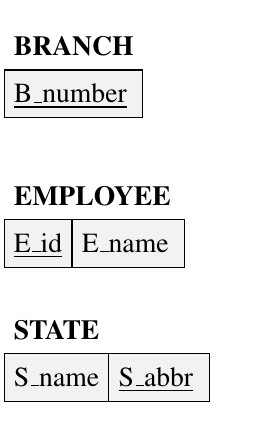
\begin{tikzpicture}[relation/.style={rectangle split,
      rectangle split parts=#1,
      rectangle split part align=base,
      draw,
      anchor=center,
      align=center,
      text height=3mm,
      text centered}]
  \hspace*{-0.3cm}

  % RELATIONS

  \node (branchtitle) {\textbf{BRANCH}};

  \node[relation=1,
    rectangle split horizontal,
    rectangle split part fill={lightgray!50},
    anchor=north west,
    below=0.6cm of branchtitle.west,
    anchor=west](branch) {
    \underline{B\_number}
  };

  \node [below=1.3cm of branch.west,
    anchor=west] (employeetitle) {
    \textbf{EMPLOYEE}
  };


  \node [relation=2,
    rectangle split horizontal,
    rectangle split part fill={lightgray!50},
    below=0.6cm of employeetitle.west,
    anchor=west] (employee) {
    \underline{E\_id}%
    \nodepart{two} E\_name
  };

  \node [below=1.1cm of employee.west,
    anchor=west] (statetitle) {
    \textbf{STATE}
  };


  \node [relation=2,
    rectangle split horizontal,
    rectangle split part fill={lightgray!50},
    anchor=north west,
    below=0.6cm of statetitle.west,
    anchor=west] (state) {
    S\_name%
    \nodepart{two}   \underline{S\_abbr}
  };

\end{tikzpicture}
\vspace{0.3cm}


\subsection*{Step 2: Mapping of Weak Entity Types}
In the second step, weak entities were mapped. This resulted in the relation CITY. The primary key for CITY was composed from the primary key of it's owner entity, STATE (Abbreviation as `S\_abbr'), and it's partial key `City Name' as `C\_name'.

\vspace{0.3cm}
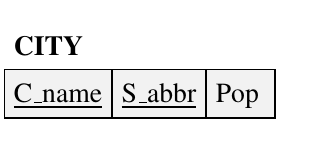
\begin{tikzpicture}[relation/.style={rectangle split,
      rectangle split parts=#1,
      rectangle split part align=base,
      draw,
      anchor=center,
      align=center,
      text height=3mm,
      text centered}]
  \hspace*{-0.3cm}

  % RELATIONS

  \node (citytitle) {\textbf{CITY}};

  \node[relation=3,
    rectangle split horizontal,
    rectangle split part fill={lightgray!50},
    anchor=north west,
    below=0.6cm of citytitle.west,
    anchor=west](city) {
    \underline{C\_name}
    \nodepart{two} \underline{S\_abbr}
    \nodepart{three} Pop
  };

\end{tikzpicture}
\vspace{0.3cm}

\subsection*{Step 3: Mapping of Binary 1:1 Relationship Types}
Now all binary 1:1 relationships were mapped. First the relationship `Manages' was mapped. `MGR\_id' of BRANCH is the foreign key that refers to `E\_id', the primary key of EMPLOYEE. Further the attribute `MGR\_start\_date' was also added to the relation BRANCH. 

\vspace{0.3cm}
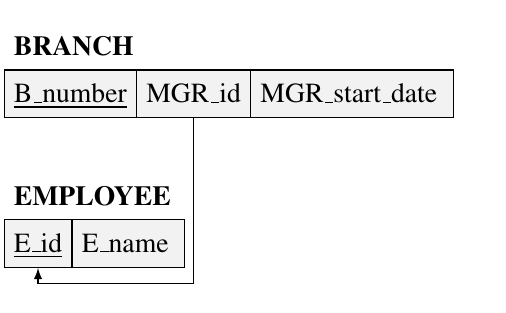
\begin{tikzpicture}[relation/.style={rectangle split, 
      rectangle split parts=#1, 
      rectangle split part align=base, 
      draw, 
      anchor=center, 
      align=center, 
      text height=3mm, 
      text centered}]
  \hspace*{-0.3cm}

% RELATIONS

  \node (branchtitle) {\textbf{BRANCH}};


  \node [relation=3, 
    rectangle split horizontal, 
    rectangle split part fill={lightgray!50}, 
    anchor=north west, 
    below=0.6cm of branchtitle.west, 
    anchor=west] (branch){ 
    \underline{B\_number}%
    \nodepart{two}   MGR\_id
    \nodepart{three} MGR\_start\_date
  };

  \node [below=1.3cm of branch.west, 
    anchor=west] (employeetitle) {\textbf{EMPLOYEE}
  };

  \node [relation=2, 
    rectangle split horizontal, 
    rectangle split part fill={lightgray!50}, 
    below=0.6cm of employeetitle.west, anchor=west] (employee) {
    \underline{E\_id}%
    \nodepart{two} E\_name
  };

  % FOREIGN KEYS

  \draw[-latex] (branch.two south) -- ++(0,-0.2) 
  -| ($(branch.two south) + (0,0)$) 
  |- ($(employee.one south) + (0,-0.20)$) 
  -| ($(employee.one south) + (0,0)$);

\end{tikzpicture}
\vspace{0.3cm}

Then the relationship `has\_capital' was mapped. `Capital' is the foreign key of STATE that refers to the primary key of CITY, `C\_name'.  

\vspace{0.3cm}
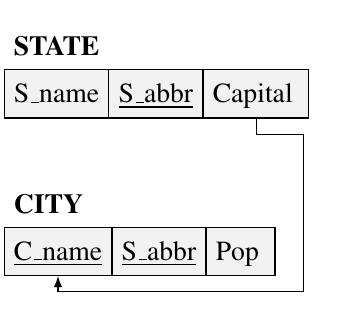
\begin{tikzpicture}[relation/.style={rectangle split, 
      rectangle split parts=#1, 
      rectangle split part align=base, 
      draw, 
      anchor=center, 
      align=center, 
      text height=3mm, 
      text centered}]
  \hspace*{-0.3cm}


  \node (statetitle) {\textbf{STATE}};

  \node [relation=3, 
    rectangle split horizontal, 
    rectangle split part fill={lightgray!50}, 
    anchor=north west, 
    below=0.6cm of statetitle.west, 
    anchor=west] (state) {
    S\_name%
    \nodepart{two}   \underline{S\_abbr}
    \nodepart{three} Capital
};

  \node [below=1.4cm of state.west, 
    anchor=west] (citytitle) {\textbf{CITY}};

  \node [relation=3, 
    rectangle split horizontal, 
    rectangle split part fill={lightgray!50}, 
    anchor=north west, 
    below=0.6cm of citytitle.west, 
    anchor=west] (city){
    \underline{C\_name}%
    \nodepart{two}   \underline{S\_abbr}
    \nodepart{three} Pop
  };

% FOREIGN KEYS

  \draw[-latex] (state.three south) -- ++(0,-0.2) 
  -| ($(state.three south) + (0.6,-0.4)$) 
  |- ($(city.one south) + (0,-0.2)$) 
  -| ($(city.one south) + (0,0)$);

\end{tikzpicture}
\vspace{0.3cm}


\subsection*{Step 4: Mapping of Binary 1:N Relationship Types}
Now the binary 1:N relationships were mapped. First for the relationship `located\_in', the primary key `C\_name' and `S\_abbr' of the CITY relation was added as foreign key to the BRANCH relation.  

\vspace{0.3cm}
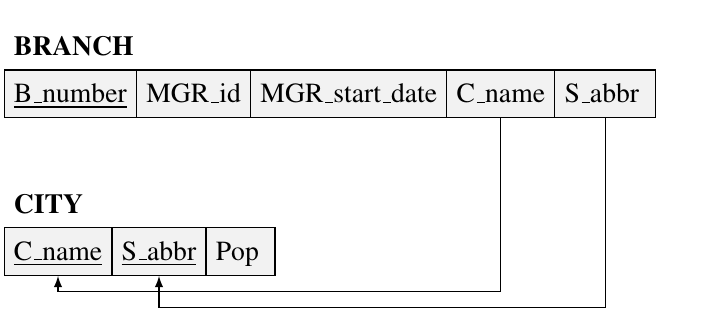
\begin{tikzpicture}[relation/.style={rectangle split, 
      rectangle split parts=#1, 
      rectangle split part align=base, 
      draw, 
      anchor=center, 
      align=center, 
      text height=3mm, 
      text centered}]
  \hspace*{-0.3cm}

% RELATIONS

  \node (branchtitle) {\textbf{BRANCH}};

  \node [relation=5, 
    rectangle split horizontal, 
    rectangle split part fill={lightgray!50}, 
    anchor=north west, 
    below=0.6cm of branchtitle.west, 
    anchor=west] (branch){ 
    \underline{B\_number}%
    \nodepart{two}   MGR\_id
    \nodepart{three} MGR\_start\_date
    \nodepart{four} C\_name
    \nodepart{five} S\_abbr
  };

  \node [below=1.4cm of branch.west, 
    anchor=west] (citytitle) {\textbf{CITY}};

  \node [relation=3, 
    rectangle split horizontal, 
    rectangle split part fill={lightgray!50}, 
    anchor=north west, 
    below=0.6cm of citytitle.west, 
    anchor=west] (city){
    \underline{C\_name}%
    \nodepart{two}   \underline{S\_abbr}
    \nodepart{three} Pop
  };

  % FOREIGN KEYS

  \draw[-latex] (branch.four south) -- ++(0,-0.2) 
  -| ($(branch.four south) + (0.0,-0.4)$) 
  |- ($(city.one south) + (1.0,-0.2)$) 
  -| ($(city.one south) + (0,0)$);

  \draw[-latex] (branch.five south) -- ++(0,-0.2) 
  -| ($(branch.five south) + (0.0,-0.4)$) 
  |- ($(city.two south) + (1.0,-0.4)$) 
  -| ($(city.two south) + (0,0)$);

\end{tikzpicture}
\vspace{0.3cm}


For the `lives\_in' relationship, `C\_name' and `S\_abbr', the primary key form the CITY relation was added as foreign key to the EMPLOYEE relation.   


\vspace{0.3cm}
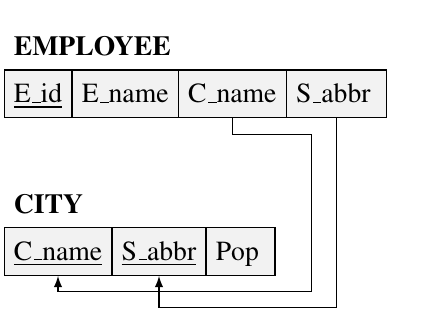
\begin{tikzpicture}[relation/.style={rectangle split, 
      rectangle split parts=#1, 
      rectangle split part align=base, 
      draw, 
      anchor=center, 
      align=center, 
      text height=3mm, 
      text centered}]
  \hspace*{-0.3cm}


  \node (employeetitle) {\textbf{EMPLOYEE}};

  \node [relation=4, 
    rectangle split horizontal, 
    rectangle split part fill={lightgray!50}, 
    below=0.6cm of employeetitle.west, anchor=west] (employee) {
    \underline{E\_id}%
    \nodepart{two} E\_name
    \nodepart{three} C\_name
    \nodepart{four} S\_abbr
  };

  \node [below=1.4cm of employee.west, 
    anchor=west] (citytitle) {\textbf{CITY}};

  \node [relation=3, 
    rectangle split horizontal, 
    rectangle split part fill={lightgray!50}, 
    anchor=north west, 
    below=0.6cm of citytitle.west, 
    anchor=west] (city){
    \underline{C\_name}%
    \nodepart{two}   \underline{S\_abbr}
    \nodepart{three} Pop
  };
  
  % FOREIGN KEYS

  \draw[-latex] (employee.three south) -- ++(0,-0.2) 
  -| ($(employee.three south) + (1.0,-0.4)$) 
  |- ($(city.one south) + (1.0,-0.2)$) 
  -| ($(city.one south) + (0,0)$);

  \draw[-latex] (employee.four south) -- ++(0,-0.2) 
  -| ($(employee.four south) + (0.0,-0.4)$) 
  |- ($(city.two south) + (1.0,-0.4)$) 
  -| ($(city.two south) + (0,0)$);


\end{tikzpicture}
\vspace{0.3cm}

Finally, the `located\_in' relationship was mapped from CITY to STATE. Each city is in exactly one state. The `has\_capital' relationship added in step three is also visible in the graph below. 


\vspace{0.3cm}
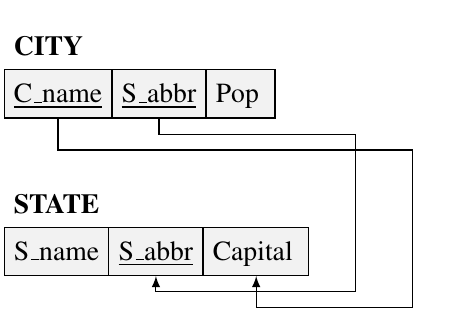
\begin{tikzpicture}[relation/.style={rectangle split, 
      rectangle split parts=#1, 
      rectangle split part align=base, 
      draw, 
      anchor=center, 
      align=center, 
      text height=3mm, 
      text centered}]
  \hspace*{-0.3cm}

  \node (citytitle) {\textbf{CITY}};

  \node [relation=3, 
    rectangle split horizontal, 
    rectangle split part fill={lightgray!50}, 
    anchor=north west, 
    below=0.6cm of citytitle.west, 
    anchor=west] (city){
    \underline{C\_name}%
    \nodepart{two}   \underline{S\_abbr}
    \nodepart{three} Pop
  };


  \node [below=1.4cm of city.west, 
    anchor=west](statetitle) {\textbf{STATE}};

  \node [relation=3, 
    rectangle split horizontal, 
    rectangle split part fill={lightgray!50}, 
    anchor=north west, 
    below=0.6cm of statetitle.west, 
    anchor=west] (state) {
    S\_name%
    \nodepart{two}   \underline{S\_abbr}
    \nodepart{three} Capital
  };



% FOREIGN KEYS

  \draw[-latex] (city.two south) -- ++(0,-0.2) 
  -| ($(city.two south) + (2.5,-0.4)$) 
  |- ($(state.two south) + (1.0,-0.2)$) 
  -| ($(state.two south) + (0,0)$);

  \draw[-latex] (city.one south) -- ++(0,-0.4) 
  -| ($(city.one south) + (4.5,-0.4)$) 
  |- ($(state.three south) + (1.0,-0.4)$) 
  -| ($(state.three south) + (0,0)$);

\end{tikzpicture}
\vspace{0.3cm}


\subsection*{Step 5: Mapping of Binary M:N Relationship Types}
To map the binary M:N relationships, a new relation `WORKS\_AT' was created. It is composed of the foreign keys `B\_number', which is the primary key of the BRANCH relation, and the foreign key `E\_id', which is the primary key of the EMPLOYEE relation. Further the attribute `Work\_start\_date' was included. 

\vspace{0.3cm}
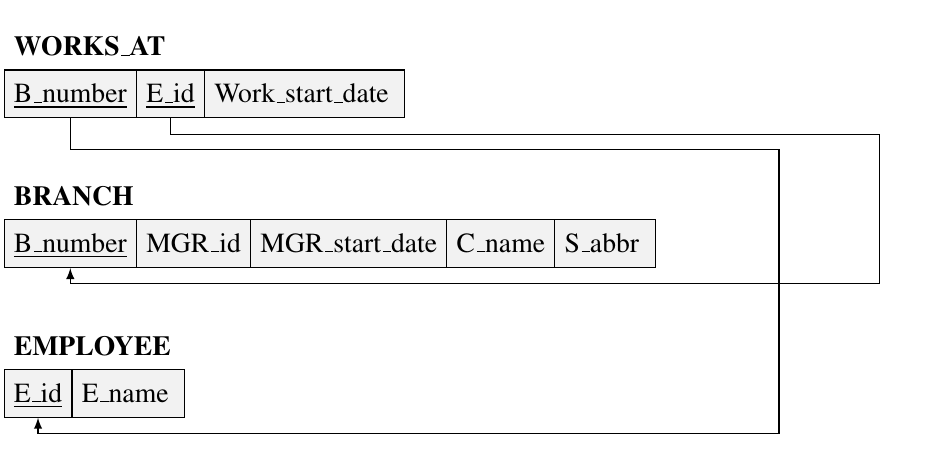
\begin{tikzpicture}[relation/.style={rectangle split, 
      rectangle split parts=#1, 
      rectangle split part align=base, 
      draw, 
      anchor=center, 
      align=center, 
      text height=3mm, 
      text centered}]
  \hspace*{-0.3cm}

  % RELATIONS

  \node (worksattitle) {\textbf{WORKS\_AT}};

  \node [relation=3, 
    rectangle split horizontal, 
    rectangle split part fill={lightgray!50}, 
    anchor=north west, 
    below=0.6cm of worksattitle.west, 
    anchor=west] (worksat){ 
    \underline{B\_number}%
    \nodepart{two}   \underline{E\_id}
    \nodepart{three} Work\_start\_date
  };

  \node [below=1.3cm of worksat.west, 
    anchor=west] (branchtitle) {\textbf{BRANCH}};


  \node [relation=5, 
    rectangle split horizontal, 
    rectangle split part fill={lightgray!50}, 
    anchor=north west, 
    below=0.6cm of branchtitle.west, 
    anchor=west] (branch){ 
    \underline{B\_number}%
    \nodepart{two}   MGR\_id
    \nodepart{three} MGR\_start\_date
    \nodepart{four} C\_name
    \nodepart{five} S\_abbr
  };



  \node [below=1.3cm of branch.west, 
    anchor=west] (employeetitle) {\textbf{EMPLOYEE}
  };

  \node [relation=2, 
    rectangle split horizontal, 
    rectangle split part fill={lightgray!50}, 
    below=0.6cm of employeetitle.west, anchor=west] (employee) {
    \underline{E\_id}%
    \nodepart{two} E\_name
  };

  % FOREIGN KEYS

  \draw[-latex] (worksat.one south) -- ++(0.0,-0.4) 
  -| ($(worksat.one south) + (9,-0.40)$) 
  |- ($(employee.one south) + (0,-0.20)$) 
  -| ($(employee.one south) + (0,0)$);

  \draw[-latex] (worksat.two south) -- ++(0.0,-0.2) 
  -| ($(worksat.two south) + (9,-0.40)$) 
  |- ($(branch.one south) + (0,-0.20)$) 
  -| ($(branch.one south) + (0,0)$);

  
\end{tikzpicture}
\vspace{0.3cm}



\subsection*{Step 6: Mapping of Multivalued Attributes}
As last step for the current ER-diagram, a new relation was created for the multivalued attribute SERVICE with the foreign key `B\_number', the primary key of the relation BRANCH. Hence a branch can have many different services.  

\vspace{0.3cm}
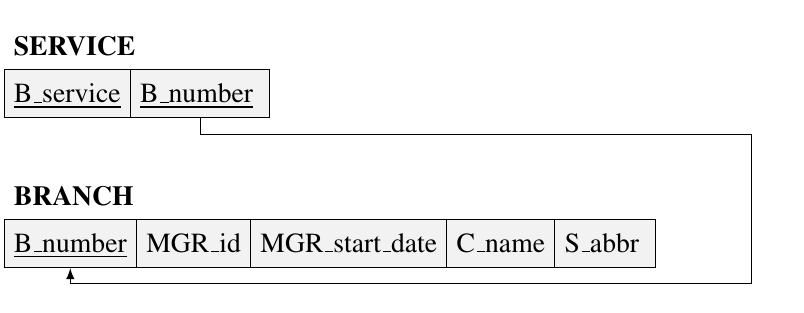
\begin{tikzpicture}[relation/.style={rectangle split, 
      rectangle split parts=#1, 
      rectangle split part align=base, 
      draw, 
      anchor=center, 
      align=center, 
      text height=3mm, 
      text centered}]
  \hspace*{-0.3cm}

  % RELATIONS

  \node (servicetitle) {\textbf{SERVICE}};

  \node [relation=2, 
    rectangle split horizontal, 
    rectangle split part fill={lightgray!50}, 
    anchor=north west, 
    below=0.6cm of servicetitle.west, 
    anchor=west] (service){ 
    \underline{B\_service}%
    \nodepart{two}  \underline{B\_number}
  };

  \node [below=1.3cm of service.west, 
    anchor=west] (branchtitle) {\textbf{BRANCH}};

  \node [relation=5, 
    rectangle split horizontal, 
    rectangle split part fill={lightgray!50}, 
    anchor=north west, 
    below=0.6cm of branchtitle.west, 
    anchor=west] (branch){ 
    \underline{B\_number}%
    \nodepart{two}   MGR\_id
    \nodepart{three} MGR\_start\_date
    \nodepart{four} C\_name
    \nodepart{five} S\_abbr
  };

    
  \draw[-latex] (service.two south) -- ++(0.0,-0.2) 
  -| ($(service.two south) + (7,-0.40)$) 
  |- ($(branch.one south) + (0,-0.20)$) 
  -| ($(branch.one south) + (0,0)$);

\end{tikzpicture}
\vspace{0.3cm}

\subsection*{Step 7: Mapping of N-ary Relationship Types}
The ER-diagram of the present exercise does not have any N-ary relationsships, hence, there was nothing to do for step 7. 



\section{Final Results}

Finally, the found relations and keys from above were condensed into one combined representation. 

\vspace{0.3cm}
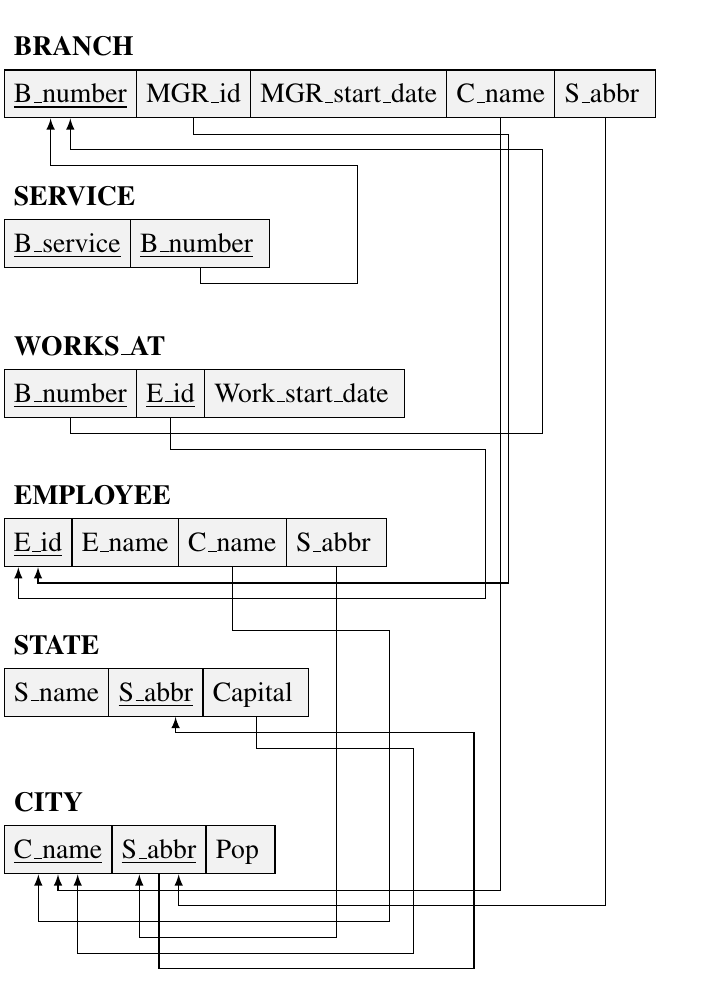
\begin{tikzpicture}[relation/.style={rectangle split, 
      rectangle split parts=#1, 
      rectangle split part align=base, 
      draw, 
      anchor=center, 
      align=center, 
      text height=3mm, 
      text centered}]
  \hspace*{-0.3cm}


  \node (branchtitle) {\textbf{BRANCH}};

  \node [relation=5, 
    rectangle split horizontal, 
    rectangle split part fill={lightgray!50}, 
    anchor=north west, 
    below=0.6cm of branchtitle.west, 
    anchor=west] (branch){ 
    \underline{B\_number}%
    \nodepart{two}   MGR\_id
    \nodepart{three} MGR\_start\_date
    \nodepart{four} C\_name
    \nodepart{five} S\_abbr
  };


  \node [below=1.3cm of branch.west, 
    anchor=west] (servicetitle) {\textbf{SERVICE}};

  \node [relation=2, 
    rectangle split horizontal, 
    rectangle split part fill={lightgray!50}, 
    anchor=north west, 
    below=0.6cm of servicetitle.west, 
    anchor=west] (service){ 
    \underline{B\_service}%
    \nodepart{two}   \underline{B\_number}
  };

  
  \node [below=1.3cm of service.west, 
    anchor=west] (worksattitle) {\textbf{WORKS\_AT}};

  \node [relation=3, 
    rectangle split horizontal, 
    rectangle split part fill={lightgray!50}, 
    anchor=north west, 
    below=0.6cm of worksattitle.west, 
    anchor=west] (worksat){ 
    \underline{B\_number}%
    \nodepart{two}   \underline{E\_id}
    \nodepart{three} Work\_start\_date
  };


  \node [below=1.3cm of worksat.west, 
    anchor=west] (employeetitle) {\textbf{EMPLOYEE}
  };

  \node [relation=4, 
    rectangle split horizontal, 
    rectangle split part fill={lightgray!50}, 
    below=0.6cm of employeetitle.west, anchor=west] (employee) {
    \underline{E\_id}%
    \nodepart{two} E\_name
    \nodepart{three} C\_name
    \nodepart{four} S\_abbr
  };


  \node [below=1.3cm of employee.west, 
    anchor=west] (statetitle) {\textbf{STATE}};

  \node [relation=3, 
    rectangle split horizontal, 
    rectangle split part fill={lightgray!50}, 
    anchor=north west, 
    below=0.6cm of statetitle.west, 
    anchor=west] (state) {
    S\_name%
    \nodepart{two}   \underline{S\_abbr}
    \nodepart{three} Capital
};

  \node [below=1.4cm of state.west, 
    anchor=west] (citytitle) {\textbf{CITY}};

  \node [relation=3, 
    rectangle split horizontal, 
    rectangle split part fill={lightgray!50}, 
    anchor=north west, 
    below=0.6cm of citytitle.west, 
    anchor=west] (city){
    \underline{C\_name}%
    \nodepart{two}   \underline{S\_abbr}
    \nodepart{three} Pop
  };

  \draw[-latex] (branch.two south) -- ++(0.0,-0.2) 
  -| ($(branch.two south) + (4,-0.40)$) 
  |- ($(employee.one south) + (0,-0.20)$) 
  -| ($(employee.one south) + (0,0)$);

  \draw[-latex] (branch.four south) -- ++(0.0,-0.3) 
  -| ($(branch.four south) + (0,-0.40)$) 
  |- ($(city.one south) + (0,-0.20)$) 
  -| ($(city.one south) + (0,0)$);

  \draw[-latex] (branch.five south) -- ++(0.0,-0.4) 
  -| ($(branch.five south) + (0,-0.40)$) 
  |- ($(city.two south) + (0.25,-0.40)$) 
  -| ($(city.two south) + (0.25,0)$);

  \draw[-latex] (worksat.one south) -- ++(0.0,-0.2) 
  -| ($(worksat.one south) + (6,+0.40)$) 
  |- ($(branch.one south) + (0,-0.40)$) 
  -| ($(branch.one south) + (0,0)$);

    \draw[-latex] (worksat.two south) -- ++(0.0,-0.4) 
  -| ($(worksat.two south) + (4,-0.40)$) 
  |- ($(employee.one south) + (0,-0.40)$) 
  -| ($(employee.one south) + (-0.25,0)$);


  \draw[-latex] (service.two south) -- ++(0.0,-0.2) 
  -| ($(service.two south) + (2,+0.40)$) 
  |- ($(branch.one south) + (0,-0.60)$) 
  -| ($(branch.one south) + (-0.25,0)$);

  \draw[-latex] (employee.three south) -- ++(0.0,-0.8) 
  -| ($(employee.three south) + (2,-0.80)$) 
  |- ($(city.one south) + (0,-0.60)$) 
  -| ($(city.one south) + (-0.25,0)$);

  \draw[-latex] (employee.four south) -- ++(0.0,-0.6) 
  -| ($(employee.four south) + (0,-0.40)$) 
  |- ($(city.two south) + (0,-0.80)$) 
  -| ($(city.two south) + (-0.25,0)$);

  \draw[-latex] (city.two south) -- ++(0,-1.2) 
  -| ($(city.two south) + (4.0,-1.2)$) 
  |- ($(state.two south) + (4.0,-0.2)$) 
  -| ($(state.two south) + (0.25,0)$);

  \draw[-latex] (state.three south) -- ++(0.0,-0.4) 
  -| ($(state.three south) + (2,-0.4)$) 
  |- ($(city.one south) + (0.25,-1.0)$) 
  -| ($(city.one south) + (0.25,0)$);

\end{tikzpicture}
\vspace{0.3cm}


\addcontentsline{toc}{section}{\refname}
%\bibliography{references}

\end{document}
